\subsubsection{Comando PUT}
Nel messaggio di comando put, dopo i primi 8 bit che specificano il comando, 
seguono: il nome del file delimitato dal terminatore di stringa, la dimensione
del file in un campo di 64 bit ed infine il file stesso.
	%+-------+-----------------------+---------------------------+-----------------------------------+
	%|  PUT  |	   file_name     	|		  file_size         |	..			file			..	|
	%+-------+-----------------------+---------------------------+-----------------------------------+
	%  8 bit										64 bit
\begin{figure}[!h]
	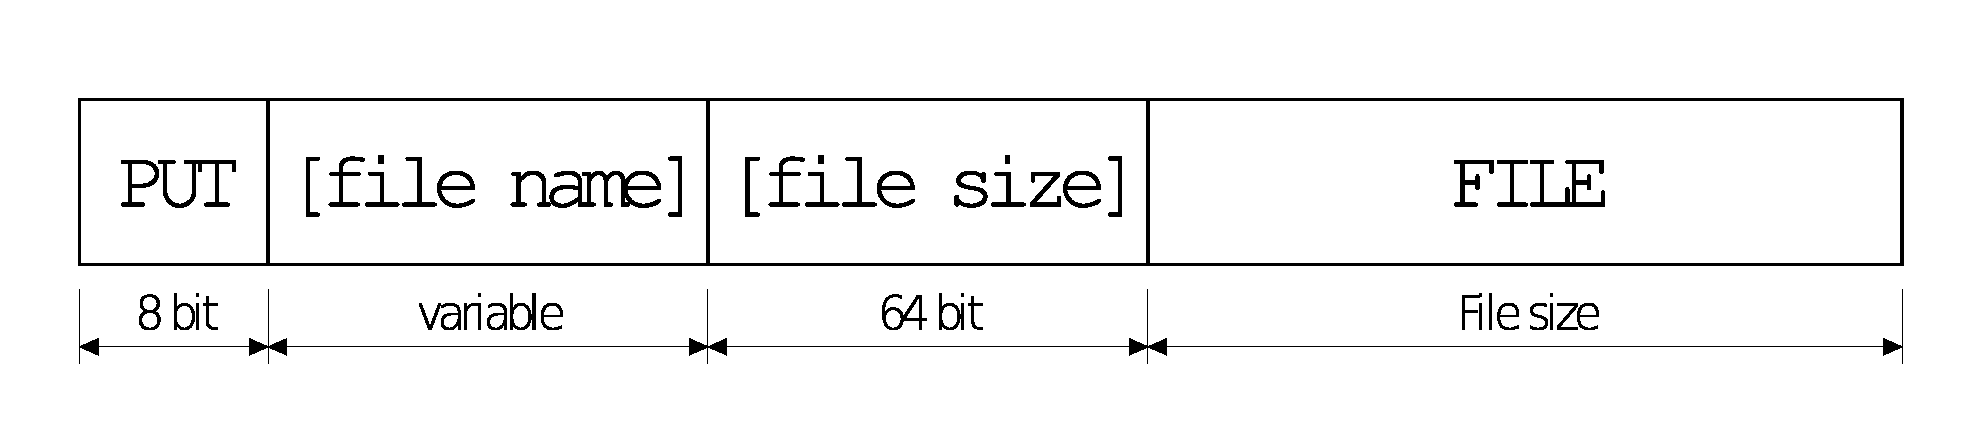
\includegraphics[scale=0.35]{images/put_client}
	\caption{Messaggio di comando PUT}
\end{figure}
Il server avvia la procedura di ricezione al termine della quale invia indietro
un messaggio di 8 bit con l'esito dell'operazione.
	%+-----------+							+-----------+
    %|PUT_SUCCESS|         oppure            |PUT_FAILURE|
    %+-----------+                           +-----------+
	%	8 bit									8 bit
\begin{figure}[!h]
	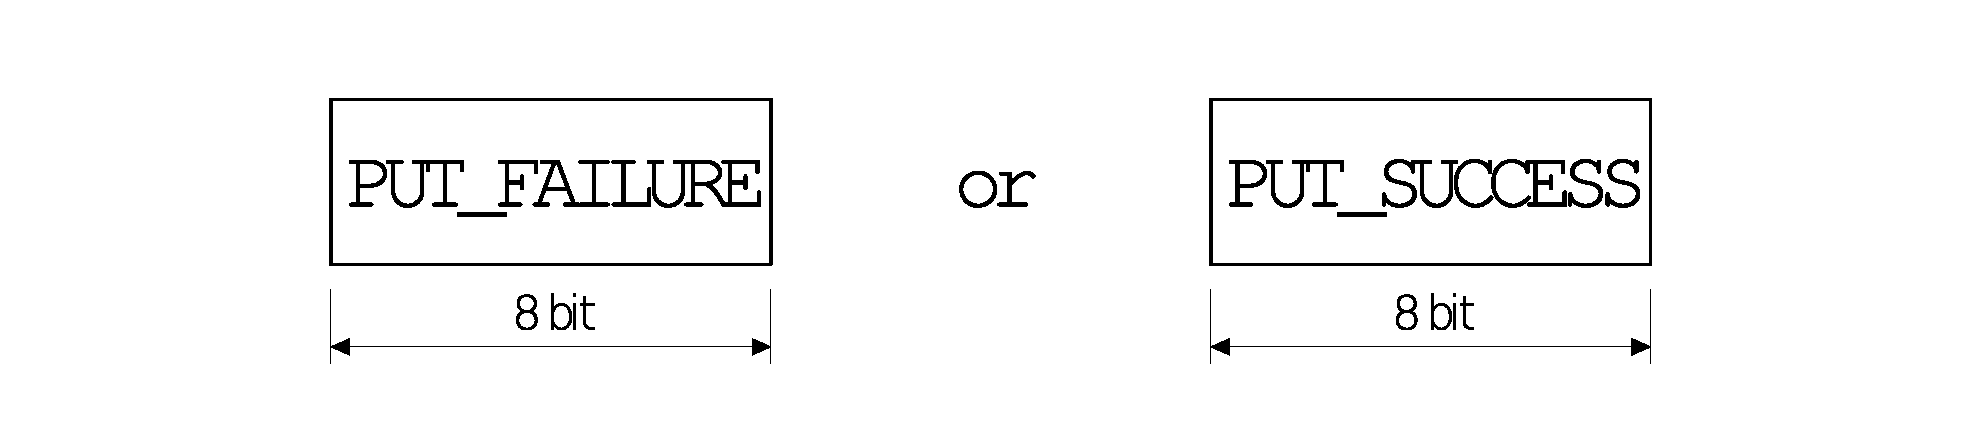
\includegraphics[scale=0.35]{images/put_server}
	\caption{Messaggio di risposta PUT}
\end{figure}
